\begin{abstract}
In a series of two events regarding privacy, a large number of users migrated from WhatsApp to other instant messaging platforms.
This essay explores this case of channel choice through the lenses of media richness theory, social influence model and concludes that a combination of them, dual capacity model, explains the results of this incident the best.
Through a slight modification of DCM, we can soundly conclude that the choice on WhatsApp's side was inadequate.
The focus of the analysis is on (1) failure of communication from WhatsApp and (2) subsequent user channel choice.
\end{abstract}

\section{Introduction}

% \TODO{add explicit task requirements/properties and channel characteristics}

WhatsApp is an instant messaging service that also supports voice and video calls and sharing of multimedia content.
In two events, acquisition by Facebook and policy renewal, many users reconsidered their choices of using this communication channel and switched to other platforms.
This essay takes the merger with Facebook and the initial backlash into consideration, though is concerned more with the more recent policy renewal and its effect.
I conclude that WhatsApp failed to clearly communicate the necessity of policy renewal through the analysis via media richness theory \citep{daft1983information}, social influence model \citep{fulk1990social} and dual capacity model \citep{sitkin1992dual}.
Many users were confused about the interpretation of the message and perceived it as dishonest, which was further fueled by breaking prior promises.
The fact that this message of policy renewal was communicated to everyone at the same time and was highly medialized was a key factor that gave rise to the opportunity of many social circles to migrate to different platforms.

\paragraph{Outline.}
To provide context, in \Cref{sec:whatsapp} I present the factual account of the development of events related to WhatsApp privacy together with a summary of related works in \Cref{subsec:whatsapp_prior}.
This is followed up with an analysis of communication patterns and the effect of the latest event on user channel choice in \Cref{sec:analysis}.
Generalizing remarks and conclusion are presented in \Cref{sec:discussion,sec:conclusion}.

% metadata paragraph here VERY GOOD!
% https://arxiv.org/pdf/1701.06817.pdf

\section{WhatsApp Privacy} \label{sec:whatsapp}

\subsection{Prior concerns} \label{subsec:whatsapp_prior}

The issues regarding WhatsApp privacy have mostly been studied with respect to the technical and implementational aspects \citep{terpstra2013whatsapp,carpay2019whatsapp,abiodun2020reinforcing}.
\citet{rastogi2017whatsapp} conclude that despite WhatsApp being technically secure because of the use of end-to-end encryption, metadata are left unencrypted and accessible by the app provider.
This is usually followed up by discussions related to government back-door access and national security \citep{endeley2018end}.

Non-technical literature is mostly concerned about the privacy concerns that arise within the use and between users.
\citet{santos2020analyzing} identified the following such issues: (1) sharing private information (phone number, online status, read receipts) to other users and within groups and (2) forwarding messages which may contain personal identifying information with unlimited dissemination and exposure.
\citet{terpstra2013whatsapp} adds that even though the name can not be inferred only by the phone number, profile photos can be accessed by anyone who knows the correct phone number.
\citet{santos2020analyzing} also note the need for a shift in the perception of this channel.
Instead of viewing it either as solely public or private space (belonging to the user), but rather as a shared space.

\citet{sutikno2016whatsapp} and \citet{rosler2018more} compare WhatsApp with other instant messaging services (Signal, Telegram, Viber and Threema).
They conclude that WhatsApp's dominant position on the market is largely due to its simplicity and being backed by its parent company, Facebook.
\citet{schreiner2015examining} attempted to model the user behaviour of switching between the services.
They conclude that privacy concerns play a vital role in switching and that dissatisfaction with WhatsApp privacy protection is a higher factor than the attraction of privacy protection of another service.

Finally, ethical concerns have been raised about the use of WhatsApp and other instant messaging apps in the context of professional and personal life.
The cost of availability and networked connections is the collapse of boundaries and reduced freedom and autonomy.
They also note that privacy infringements happen especially if the user is not aware of the specific features and functionalities.

\subsection{Acquisition \& Policy Renewal}

\paragraph{Acquisition.}
In February 2014, WhatsApp was acquired by Facebook, one of the world's most valuable technology companies.
This merger was particularly interesting because of the conflicting privacy policies of Facebook and WhatsApp \citep{esayas2017competition}.
The initial funding model of WhatsApp was a yearly subscription, which changed after the acquisition.
The funding model of Facebook is reliant on targeted advertising, a practice that becomes more effective with having access to various forms of user data.
Such metadata usage of WhatsApp has been the major source of concerns \citep{rastogi2017whatsapp}.
The public image of WhatsApp in the context of privacy consideration has been further stained by accusations of unfair and aggressive commercial practices to make the users agree to its changed new terms of services \citep{zingales2017between}.
Importantly, shortly after this merger for legal and public relations reasons, WhatsApp promised not to share consumer data with its parent company and other third parties.
This should apply to the phone numbers, contact numbers and metadata and was later breached by the company.

\paragraph{Policy Renewal.}

In January 2021, WhatsApp updated its policy, among other things, to be able to share hardware and transaction metadata with Facebook.
This was highly medialized and many users, without reading the updated privacy policy in detail, misinterpreted it as WhatsApp sharing their messages and other information with Facebook.
The backlash was greater than when WhatsApp was being merged into Facebook and as a consequence, WhatsApp's reputation plummeted and many of its users were looking to switch to other platforms.

\paragraph{Mitigation.}
WhatsApp decided on the two following measures as part of damage control.

\begin{itemize}
\item
After the realization that many people were misinformed about the implications of policy renewal, WhatsApp decided to delay the rollout date of the new changes a month later.
This was done in order to give the users more time to understand the changes in the new policy.
\item
WhatsApp launched an international campaign aimed at stressing that users' messages were end-to-end encrypted and that the new changes would not allow it to change more data with its parent company.
\end{itemize}

Even though by this time the other platforms, most notably Telegram and Signal, established a large userbase, this mitigation was effective and prevented even higher losses.

\section{Communication Analysis} \label{sec:analysis}

\subsection{WhatsApp Communication}

One of the reasons that caused the transition of users is the use of the blanket term ,,privacy issues'' which can be associated more easily with the idea of someone having access to the messages.
In the case of WhatsApp, the term referred to its sharing the metadata with Facebook.
This is a privacy issue as well, though not of the same severity as unsecured messages.
The mitigation strategy employed by WhatsApp focused on this distinction and the secondary privacy issue related to metadata was not addressed.
These are two orthogonal issues and it is reasonable to assume that people who became dissatisfied with WhatsApp belonged to at most one of the groups.
The rationale for this is that the issue with metadata use is perceived to be a problem mostly for technologically savvy users who would probably not misinterpret the original message while other users may not be aware of the issues connected to metadata usage and targeted advertising.
A small scale experiment \citep{dev2018understanding} indicated that roughly half the users are aware that their metadata is being used for advertisement purposes.

\paragraph{Media Richness Theory.}
The requirements of the task to convey the message of policy change, especially in the sensitive and controversial context of privacy, would preferably include rich media.
This is partly because of the belief prior of deception on the side of WhatsApp and, more importantly, high ambiguity of the term ,,privacy issues''.
The situation was then highly ambiguous, though with reasonably low uncertainty.

The space for channel selection itself from the point of view of WhatsApp is however very limited because it is not possible for WhatsApp employees to e.g. schedule a call with every user, nor even offer this service per demand.
The only distinction from the point of view of MRT and permissible given the limits of the distribution channel via the application is a personalization of the message.
A strategy, that WhatsApp could have employed could be to foresee this ambiguity in combination with the restriction to low-richness media and perform an in-house experiment on how this message is perceived and what possible misunderstandings may arise.
This would allow WhatsApp to fine-tune the message to prevent incorrect interpretations.

\paragraph{Social Influence Model.}
SIM assumes that media perception is subjective and socially constructed.
The failure of WhatsApp can be, in part, attributed to the violation of one of the explicit claims of SIM, namely that highly involving tasks (e.g. conflict and negotiation) are best completed using high social presence media (e.g. face-to-face).
As noted previously, this was not possible in this case, though some partial solutions were available.
SIM is also better suited because of the inherent conflict (though not interpersonal one) in this scenario: WhatsApp is delivering an ultimatum to the user to which they must agree unless they wish to stop using the service.

In contrast to MRT, SIM takes into account the circumstances of notifying of the policy renewal.
WhatsApp had the experience of the merge with Facebook with tolerable user loss.
After General Data Protection Regulation came into effect (enforceable since 2018), policy updates and notifications became omnipresent on the web.
This could lead the WhatsApp executives to believe that their policy renewal would be a routine task that required little attention and would go mostly unnoticed.
SIM categorizes the media use history as one of the contributing factors to channel choice and therefore explains the motivation for this channel use from the side of WhatsApp.

\paragraph{Dual Capacity Model.}

Neither MRT nor SIM take into account the societal impact of this message, the resonation within the public media and the creation of backchannels and as such, a theory more focused on the societal dynamics and the message receiver is needed.
DCM describes the data and symbol carrying capacities of the media and takes the recipient's cognitive and affective responses into account.

From the point of view of data-carrying capacity, the use of bulk messages was inadequate because of the high ambiguity of the situation.
The symbol carrying capacity of this medium is also lacking for this purpose because it suggests that the transferred message is not of high importance to the sender and that the balance of power is made clear by the inability of the user to reject the new changes.
WhatsApp's position may have been justified though they did not communicate their values such as their financial strategy and goals clearly to the users.
This resulted in a perception of deceit regarding metadata collection and usage.
The lack of communication of values further created a space for increased suspicion and worst-scenario interpretation (e.g. of the term privacy).
This is in alignment with the prediction of DCM that affective responses are more strongly influenced by the symbolic features of the channel (or their lack of) than the data-carrying capacity.

\begin{figure}[ht]
\centering
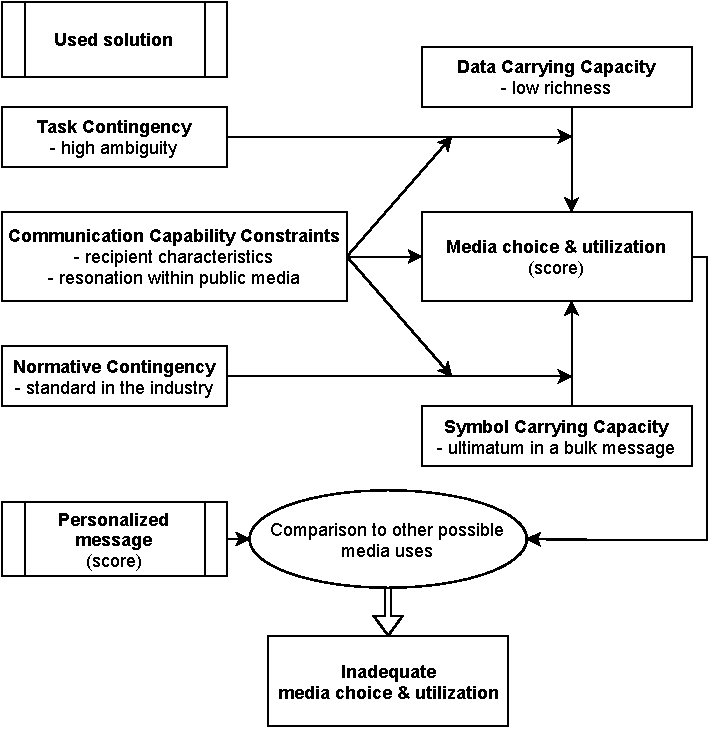
\includegraphics[width=0.77\linewidth]{img/dcm_whatsapp_choice.pdf}
\caption{Concretization of Dual Channel Model for WhatsApp policy renewal communication. Scoring and comparison with other choices added. Based on \textit{Figure 1: Determinants of Media Choice} \citep{sitkin1992dual}.}
\label{fig:dcm_whatsapp_choice}
\end{figure}

DCM then describes jointly both the inadequacy of the medium selection to resolve the ambiguity and also its failure of communicating the company values.
Because DCM is a descriptive model, it is not straightforward to reach this conclusion.
In order to conclude that a channel choice and use was inadequate, it has to be worse than any other option (\textit{,,should'' implies ,,can''}) otherwise one could not know whether only the specific choice was wrong or whether any other choice would be equally bad given the circumstances.
This is an important distinction from the practical point of view of accountability.
The original DCM does not take this comparison but can be easily modified by having the output be an \textit{adequacy score} for a pair of \textit{task - channel choice and use}.
To determine whether the choice and use were good (even if leading to poor results), one then needs to simply compare these scores to other viable choices and uses.

The major influencing factors for channel choice are displayed in \Cref{fig:dcm_whatsapp_choice}, which is a specialization of the whole DCM into the context of this situation and further extended by the scoring and comparison.
Note that task contingency and communication capability constraints negatively influence the adequacy but normative contingencies (such as this communication being the standard among policy renewal communication) supports it.
Overall we can conclude that the used solution has a lower score than at least one other solution (more personalized message) and therefore was an incorrect choice on WhatsApp's side.

\subsection{Effect of Policy Renewal on Channel Choice}

Similarly to analyzing the channel choice and use of WhatsApp, we can examine the platform choice of the users.
Even though almost all instant messaging platforms provide the same richness (data-carrying capacity is constant) and the nature of messages does not change (task contingency is constant), communication capability constraints, normative contingencies and symbol carrying capacities vary greatly and because of this, models of channel choice are also applicable here.
The use of DCM, in this case, is arbitrary, though the comparison with other platforms here becomes critical because we can assume that users' behaviour can be superfluously modelled as wanting to participate in the transfer of messages on any channel with a score above some threshold and out of these viable channels they choose to most adequate one.
This threshold need not be constant and can vary based on e.g. the message properties, such as message urgency.
The key point is that this remains constant regardless of whatever platform is being used.


\begin{figure}[ht]
\centering
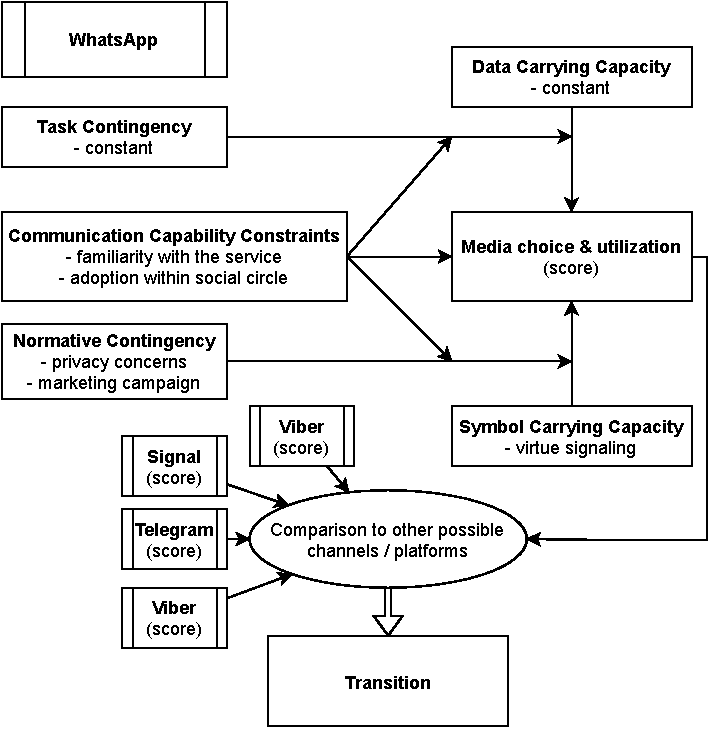
\includegraphics[width=0.77\linewidth]{img/dcm_user_choice.pdf}
\caption{Concretization of Dual Channel Model for user choice of instant messaging platform. Scoring and comparison with other choices added. Based on \textit{Figure 1: Determinants of Media Choice} \citep{sitkin1992dual}.}
\label{fig:dcm_user_choice}
\end{figure}

\Cref{fig:dcm_user_choice} depicts the situation from the point of view of the user.
If alternatives were not present or were too severely handicapped by the dominant position of WhatsApp, they would not be a viable option for most of the users that wished to transition because of the sudden negative modulation of the adequacy through privacy concerns.
WhatsApp gains its score by the inertia (familiarity with the service, reasonable expectation that the communication partner also uses the same service) and loses through (1) privacy concerns, (2) virtue signalling (i.e. someone can be seen as not caring about the ethical issues of privacy when seen using WhatsApp\footnote{In certain sociodemographic groups, such as students of cybersecurity in Germany, this was a big factor.}) and (3) prior concerns regarding the ethicality of the company and the product, as listed in \Cref{subsec:whatsapp_prior}.
Other platforms, built more upon privacy, do not suffer from this but are negatively affected by comparatively low adoption rates.

Naturally, a high transition score is not aligned with WhatsApp's goals (large adoption).
In their damage control, WhatsApp correctly identified the issue with privacy concerns and misunderstanding and launched a campaign to reverse this.
This campaign affects public opinion and as such, is part of normative contingencies that modulates the symbol carrying capacity.

\section{Discussion} \label{sec:discussion}

It is possible to theorize on why the situation was more severe when the policy was being renewed than when WhatsApp was being merged into Facebook.
I hypothesise that this is because of the raised alertness of privacy concerns in recent years, brought in part by the GDPR which became and unavoidably affected users digital experience.
This could have affected everyone who came into contact with it and primes them so that the perceptual factors in the normative contingencies group regarding privacy are higher.
In the case of the merger, it could have been too low but in the case of policy renewal, it could have reached a critical value that was enough to start the creation of backchannels and large-scale public and media speculation.

A strong assumption made in the analysis is the omission of a thorough examination of the issue by WhatsApp.
It could have been the case that an initial analysis on the possible consequences of different ways of communication was performed.
WhatsApp decision-makers could have concluded that further study would have reduced the probability of the negative reaction of the public but that this would be offset by the higher cost of performing this study.

\begin{table}[ht]
\centering
\begin{tabular}{l>{\centering\arraybackslash}p{2.35cm}>{\centering\arraybackslash}p{2.55cm}cr}
\toprule
Action (cost) & Negligible reaction $(-2)$ & Negative reaction $(-10)$ & Expected value \\
\midrule
Bulk message $(0.5)$  & $90\%$ & $10\%$ & $-2.8-0.5=\mathbf{-3.3}\leftarrow\hspace{-0.5cm}$\\
Further study $(1.5)$ & $95\%$ & $5\%$ & $-2.4-1.5=\mathbf{-3.9}$\\
\bottomrule
\end{tabular}
\caption{Possible payoff matrix for initial WhatsApp communication assessment.}
\label{tab:payoff}
\end{table}

Such a possible scenario with two outcomes and two considered strategies is shown in \Cref{tab:payoff}.
The failure of WhatsApp's communication could have then been a faulty analysis (i.e. underestimating the chance and cost of a negative reaction).
This could have stemmed from the fact that many other companies communicated their policies renewals via bulk messages and faced no significant public backlash.

The presented extension of DCM for the purpose of user platform choice reaches similar conclusions to the pull-push model \citet{schreiner2015examining} (every factor of a platform has a pull-value and push-value).
Eventually, all the scores of the platforms get compared and the prominent ones are chosen.
The advantage of simply adding scoring and comparison, as done in the updated DCM, is that it can be added to an arbitrary model of channel selection and share its assumptions and claims.

\section{Conclusion} \label{sec:conclusion}

This essay examined the issue of WhatsApp policy renewal from the view of channel choice by Media Richness Theory, Social Influence Model and Dual Capacity Model.
A slight extension to DCM (comparing with other options) showed to be the most appropriate for concluding that the choice made by WhatsApp was inadequate.
The same updated model showed to be also useful in explaining the transition of users from using WhatsApp to other instant messaging platforms.
Future works could focus on quantifying the importance of relevant factors in user instant messaging platform choice, possibly within the updated scoring model.